\chapter{
شمارنده دودویی سنکرون
}

در این قسمت باید یک مدار ترتیبی را درست کنیم که بسته به ورودی قبلی خود به یک ورودی خاص بعدی می‌رود.

مراحل انجام این کار و ساده‌سازی ورودی‌های فلیپ‌فلاپ‌ها در ادامه به شکل دست‌نویس آمده است.
خوش‌بختانه پاسخ نهایی به مقدار زیادی ساده می‌شود.

نتیجه‌ی نهایی در شکل
\eqref{fig:circuit3}
آمده است.

\begin{figure}
    \centering
    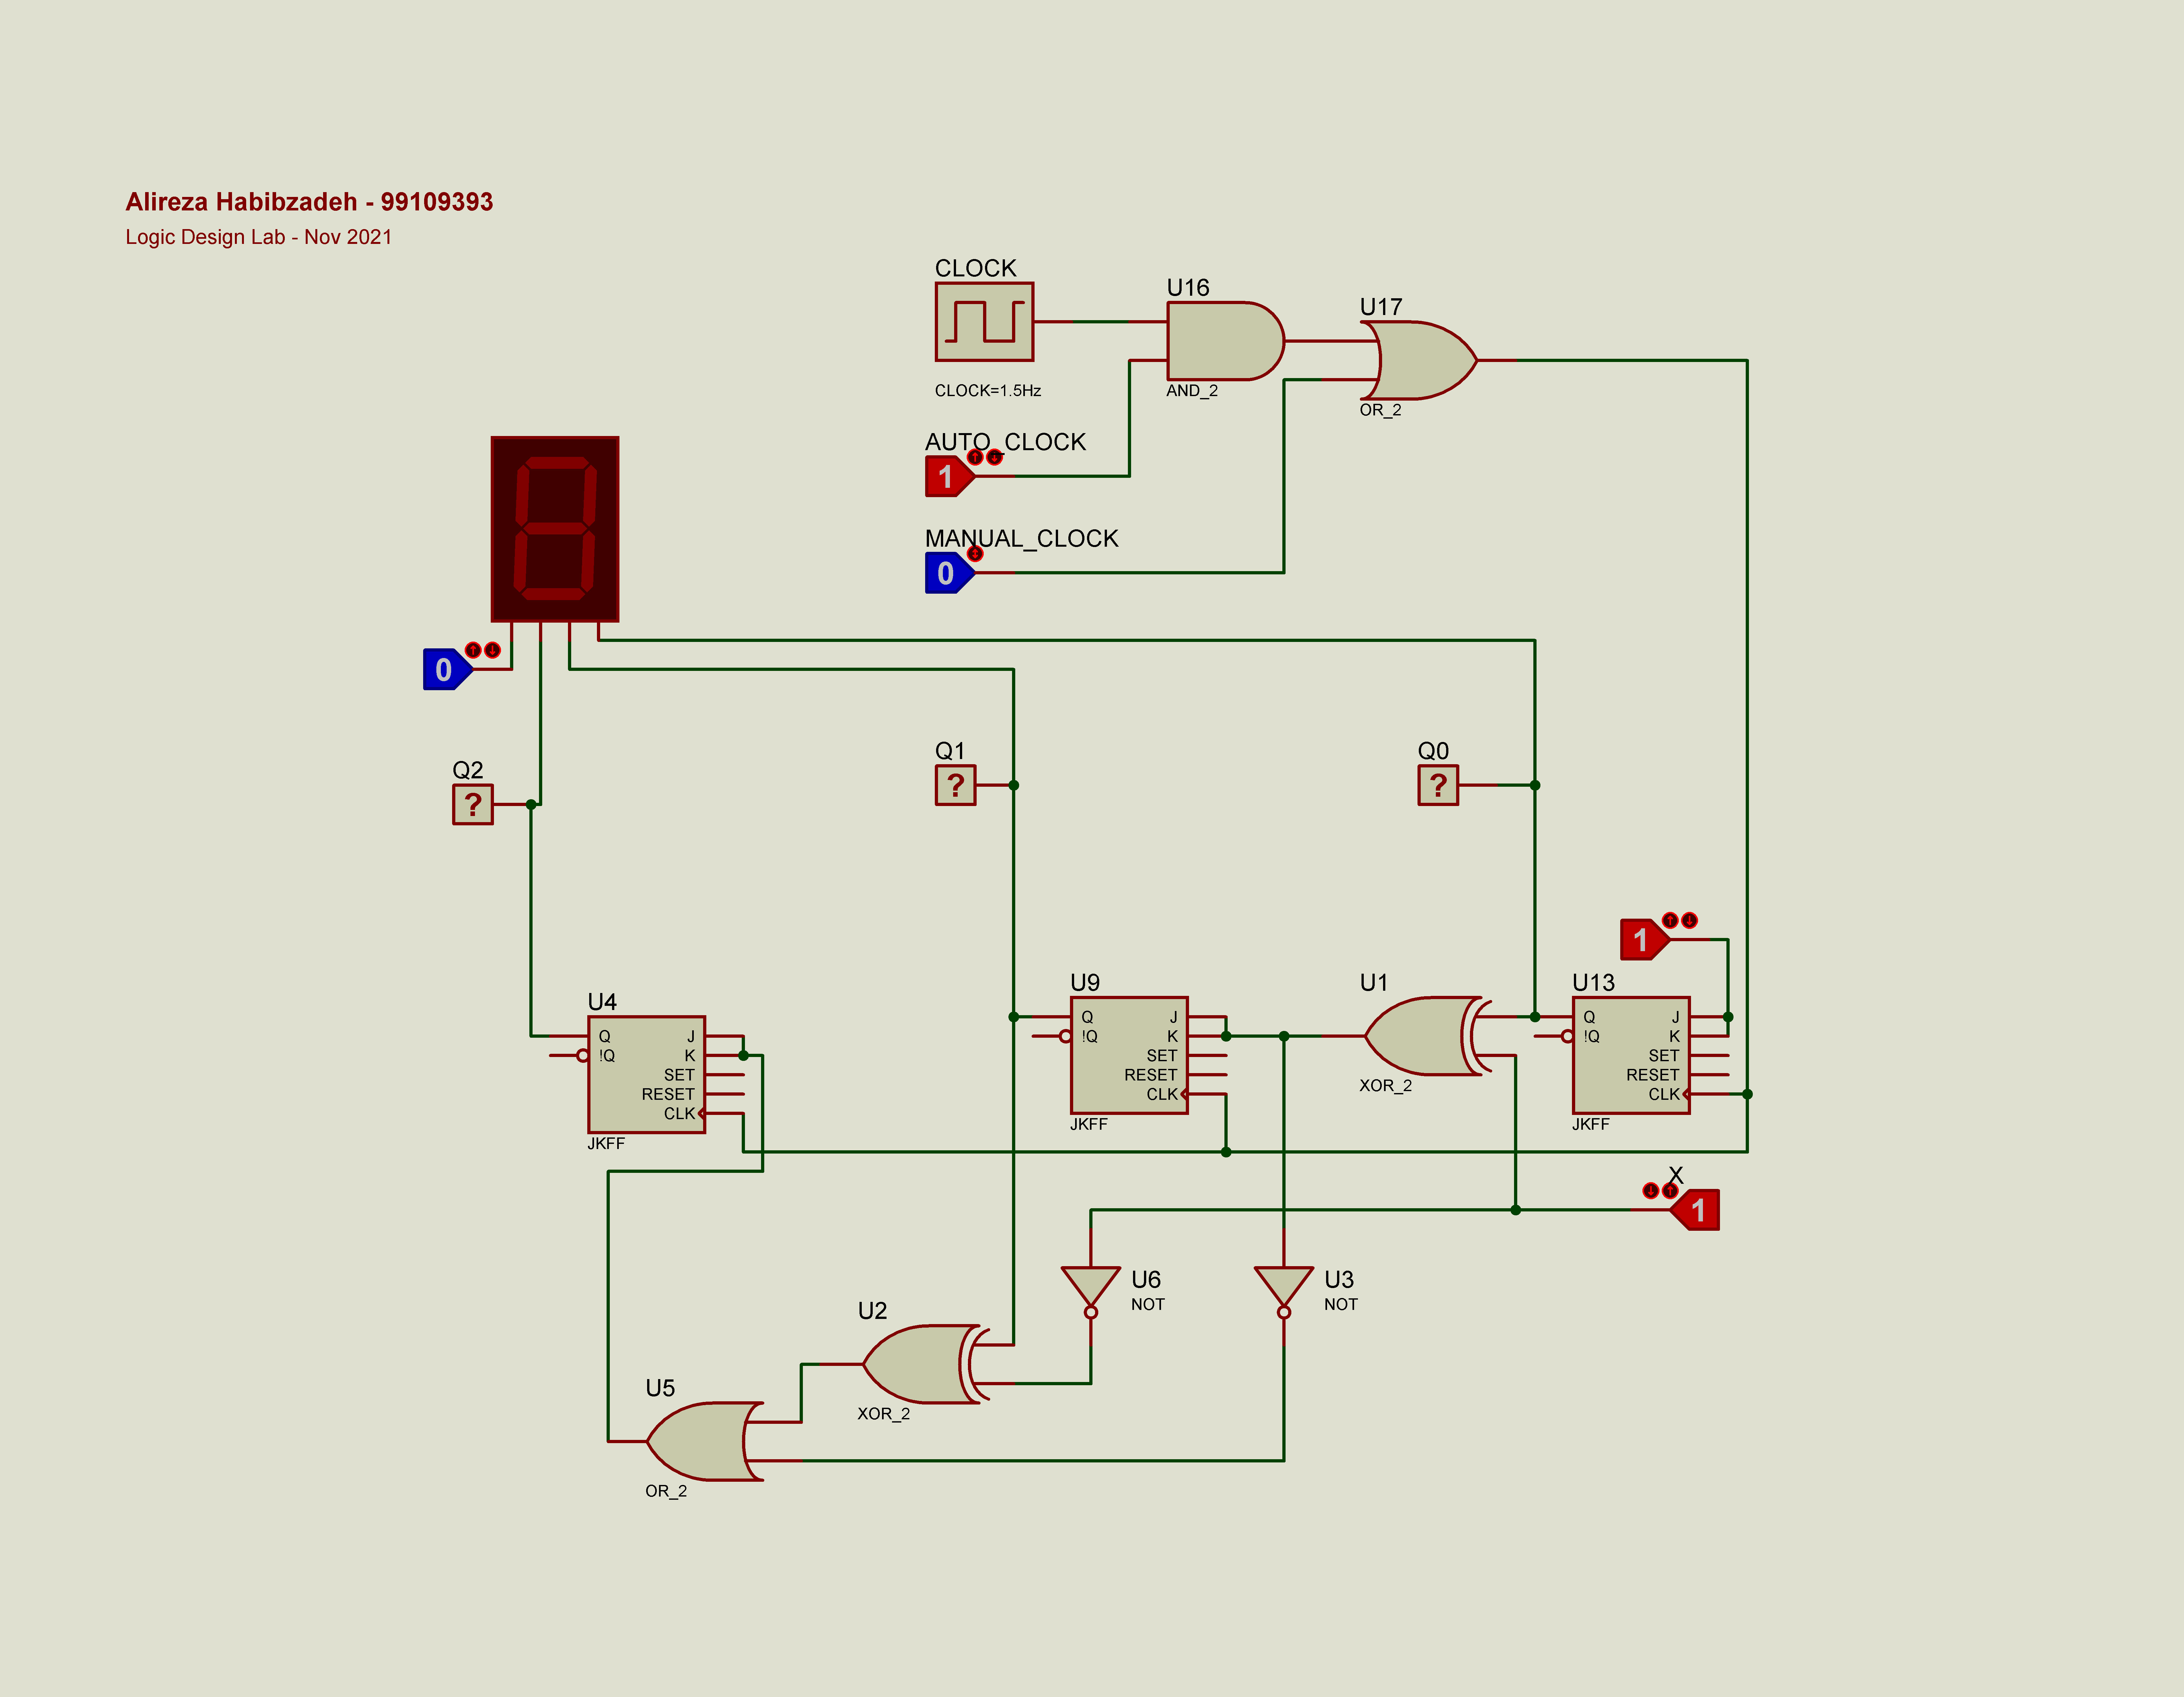
\includegraphics[width=\textwidth]{part2/image.png}
    \caption{
    شمارنده سه بیتی سه تا سه تا
    }
    \label{fig:circuit3}
\end{figure}